For the second iteration both the pathfinding and the raycasting had to be optimized since they both used to much of the CPU.

\subsection*{Optimizing pathfinding}
A way to optimize runtime performance of the pathfinding is to reduce the graph.
This would be done by creating a waypoint graph instead of a grid graph.
The waypoints would be created at the outer corners of the obstacles on the map, where the AI could make a turn, as seen in figure \ref{waypointsNode}.
Each point would then do a raycast to every other point to see if it was in direct line of sight, and if that was the case it was added as a neighbour and the cost of that edge would be the euclidean distance to that point.
A resulting graph can be seen in Figure \ref{waypointgraph}.
In comparison the old graph created had 3984 nodes and 30450 edges while this approach resulted in a much smaller graph with 47 nodes and 624 edges, thus improving both the creation and traversal times of the graph.

\begin{figure}[H]
\centering
\begin{minipage}{.5\textwidth}
\centering
	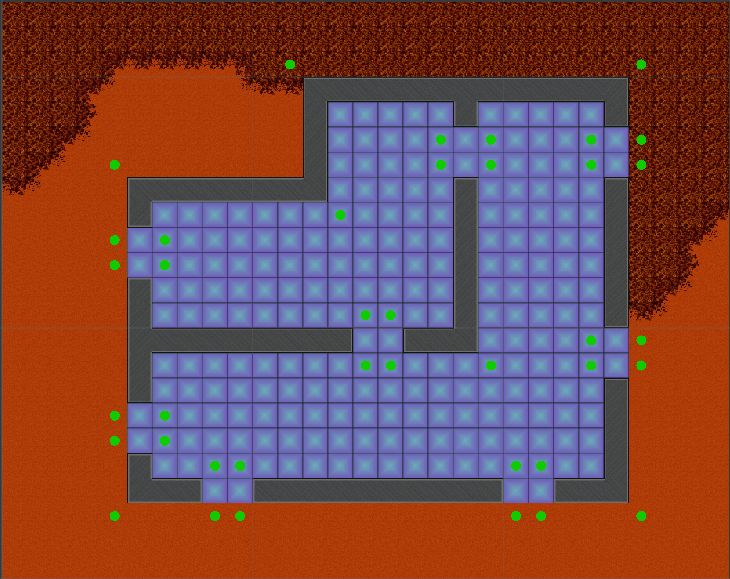
\includegraphics[width=0.9\textwidth]{figures/astar/waypoints}
	\caption{The placement of the waypoints}
	\label{waypointsNode}
	\end{minipage}%
\begin{minipage}{.5\textwidth}
\centering
	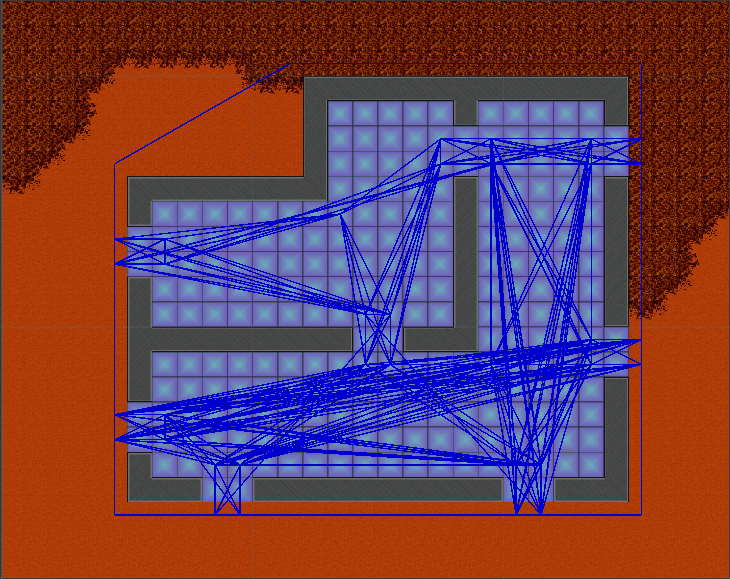
\includegraphics[width=0.9\textwidth]{figures/astar/waypointsGraph}
	\caption{Graph based on the waypoints}
	\label{waypointgraph}
	\end{minipage}
\end{figure}

This however raised a new problem, since there were fewer waypoints available the enemies had to find the nearest accessible waypoint.
To solve this the distances was calculated to each waypoint from the given position and then a ray was cast from the position of the enemy to the position of the nearest waypoint.
If the raycast hit an object the algorithm would move onto the second closest and so forth, as illustrated in Figure \ref{nearestWaypoint}.
\begin{figure}[H]
\begin{center}

	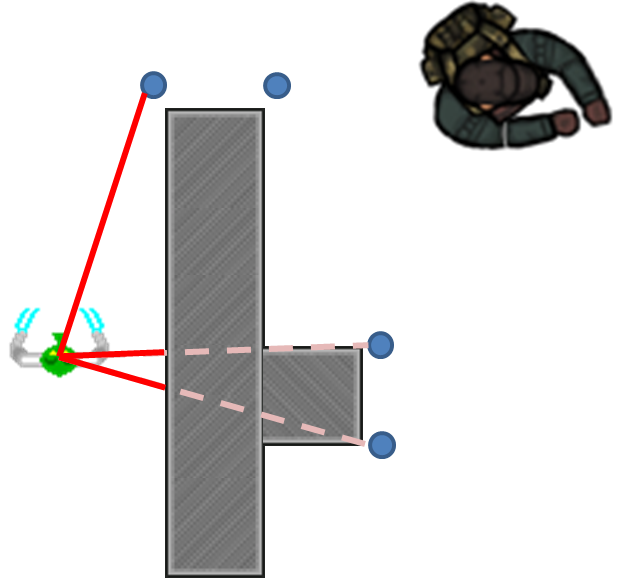
\includegraphics[width=0.4\textwidth]{figures/astar/findNearestWaypoint}
	\caption{Raycasts finding the nearest accessible waypoint. Character Art by rileygombart\cite{artist}}
	\label{nearestWaypoint}
	
\end{center}
\end{figure}

\subsection*{Minimizing of raycasting}
The minimizing of the raycasts is simply solved by adding a larger interval between each raycast.

\subsection*{Result}
While this solution had a much better performance, we found that the raycasting was still too CPU intensive and that it was desirable to remove it completely on runtime.